\documentclass[12pt]{article}
\usepackage[margin=1in]{geometry}
\usepackage{natbib}
\usepackage{graphicx}
\usepackage{caption}
\usepackage{subcaption}
\usepackage{multirow}
\usepackage{longtable}
\usepackage{color}
\bibliographystyle{apalike}

\begin{document}

\title{Genome Evolution of Domesticated of Peach and Almond}

\author{\small\sfbf{Dianne Velasco$^{\S}$, Mallikarjuna Aradhya$^{\dag}$, Jeffrey Ross-Ibarra$^{\S\ddag}$}\thanks{Corresponding author: Department of Plant Sciences, University of California, Davis, California 95616, USA. E-mail: \mbox{rossibarra@ucdavis.edu}} \\[0.3cm]
     \small\sf $^{\S}$Department of Plant Sciences, University of California, Davis, California 95616, USA,\\
     \small\sf $^{\dag}$USDA-ARS National Clonal Germplasm Repository, Davis, California 95616, USA,\\
     \small\sf $^{\ddag}$Center for Population Biology and Genome Center, University of California, Davis, California 95616, USA}

\date{\today}

\maketitle

\section*{Introduction}
\emph{Prunus} is the largest genus in the family Rosaceae with approximately four hundred species including multiple domesticated crops (almond, apricot, cherry, peach, and plum) in three of its five subgenera.
%reference to number of approximate number of species, suppose number depends on reference
%
%With over 200 species in genus Prunus subgenus Amygdalus (Rosaceae), almonds [\emph{Prunus dulcis} (Mill.) D. A. Webb], peaches [\emph{P. persica} (L.) Batsch.], and their wild relatives were originally classified solely by morphology \citep{huang20082}. 
%
%The cultivated almond (\emph{Prunus dulcis}) and peach (\emph{Prunus persica}) are just two of the over 200 species in the genus \emph{Prunus}, and both belong to the subgenus \emph{Amygdalus} (Rosaceae) along with their closest wild relatives. 
%
The subgenus \emph{Amygdalus} includes the most mophologically distinct sibling species, \emph{P. persica} (Mill.) D. A. Webb (peach) and \emph{P. dulcis} (L.) Batsch (almond).
%
%Interfertility and similar developmental morphology of almond and peach led investigators of the 18th and 19th centuries, including \citet{darwin1868variation}, to question their classification as separate species \citep{hedrick1917peaches}. 
%NOTE: somehow want to include that the species are interfertile, or somehow indicate how similar they are
%
While \emph{Prunus} species are generally outcrossing due to gametophytic self-incompatibility, though self-compatible alleles are known to exist in multiple species across the genus, peach is fully self-compatible. 
%
Domestication of almond and peach occurred approximately 5000 years ago in the Fertile Crescent and China \citep{zohary2012domestication}, respectively, followed by global dissemination \citep{hedrick1917peaches, edwards1975almond, gradziel2011origin, zheng2014archaeological}.
%
%Cultivated for thousands of years and intertwined in culture and mythology, almonds and peach remain valuable international agricultural commodities with US commercial production of more than 3.3 billion (NASS 2010).
%UPDATE: believe almond has surpassed 4 billion alone
%may not be that important
%
%Additionally peach-almond hybrids are commonly used as vigorous, pest- and disease-resistant rootstock for both crops \citep{esmenjaud1994inter}, and will continue to be important genetic resources in the face of climate change. 
%
%Interspecific hybrids of almonds, peaches, and their wild relatives are currently in use as vigorous, pest- and disease-resistant rootstock for both crops, and will continue to be important genetic resources in the face of climate change. 
%
%Almonds, for example, are drought tolerant, whereas peaches often have resistance to pests and diseases under moist conditions, due to adaptation to their xeric and mesic origins, respectively. 
%
Both domestication and mating system have been shown to significantly impact genome evolution in annual species \citep{glemin2006impact, doebley2006molecular, slotte2013capsella}. 
%
However, the manner in which domestication and mating system influence genome evolution of tree species remains poorly understood \citep{mckey2010evolutionary}.
\\
\\
%BACKGROUND ON SPECIES
%
%\emph{P. dulcis} (almond) and \emph{P. persica} (peach) are deciduous, insect pollinated trees native to a vast area extending from southern and eastern Europe through southwestern and central Asia to China, eastern and southeastern Asia, regions separated both topographically and climatically by the Himalayas and neighboring mountain ranges. 
%relates more to subgenus than these two species specifically, although post dissemination ar in those areas
%
%Almonds, for example, are distributed throughout xeric environments suggesting drought tolerance \citep{browicz1996genus}, whereas peaches often distributed in more mesic environments and have contributed resistance to pests and diseases found in these conditions \citep{beckman1998relative}, due to adaptation to their xeric and mesic origins, respectively. 
%
%Almond and peach are native to the vast geographic range extending from the eastern edge of Europe through southwestern and central Asia to China, separated both topographically and climatically by the Himalayas and neighboring mountain ranges. 
%
%Almond and peach were domesticated approximately 5000 years ago in the Fertile Crescent and China \citep{zohary2012domestication}, respectively, and subsequently disseminated globally \citep{hedrick1917peaches, edwards1975almond, gradziel2011origin, zheng2014archaeological}.
%
%With clonal propagation of peach known in China by at least 2500-2700 BP it was likely disseminated both clonally and by seed and with its self-compatible nature also meant little reduction in fruit production during dissemination.
%peach clonal propagation likely due to ease of rootability
%believe the Chinese records are from the Spring and Autumn Annals, records from the period 722-481 BC
%
%In contrast, not only is almond difficult to clonally propagate, it is self-incompatible and therefore thought to have been disseminated via seed despite the chance of offspring with bitter kernels. 
%Browicz and Zohary for almond
%
In addition to having a similar length of domestication, peach and almond are also similar in early fruit development, perenniality, precocity, genome organization \citep{arus2012peach}, and genome size \citep{arumuganathan1991nuclear, dickson1992nuclear, baird1994estimating,  loureiro2007two}.
%
Most striking however are their obvious differences in mature fruit morphology and mating systems, but almond and peach also differ in life span (longer v. shorter), chilling requirements (lower v. higher) and adventitious root generation (poor v. good).
%
The few obvious traits associated with domestication in almond are reduced toxicity, thinner endocarp, and increased seed size, while domestication traits in peach are characterized by diverse fruit morphology (size, color, texture, shape, etc.) and self-compatibility.
%
However, other traits associated with both almond and peach, such as precocity, or solely with peach, such as relative ease of adventitious rooting, may have also been targeted or incidentally selected during domestication. 
%
%Recent studies attempting to resolve the relationship of almond, peach and their wild relatives in subgenus \emph{Amygdalus} \citep{bortiri2001phylogeny, martinez2003relationships,aradhya2004molecular, oh2005molecular, zeinalabedini2010origin, delplancke2012gene, rahemi2012genetic, yazbek2013peaches}. 
%
Unfortunately, efforts to identify the wild progenitors of almond and peach \citep{verde2013high, aradhya2004molecular, zeinalabedini2010origin, mowrey1990isozyme, browicz1996genus, ladizinsky1999origin, bassi20081} have had mixed results. 
%The phylogenetic uncertainty and interfertility among many species in subgenus \emph{Amygdalus} have hindered 
%
Given the uncertainty identifying wild progenitors of almond and peach, domestication studies using crossing experiments are particularly difficult in addition to being generally impractical with long-lived perennial species.
%\citep{verde2013high, aradhya2004molecular, zeinalabedini2010origin, mowrey1990isozyme, browicz1996genus, ladizinsky1999origin, bassi20081}
%citation for crossing experiments doesn't quite seem to fit, perhaps one of Doebley's papers or others using domesticated x wild cross to identify loci
%
%Originally all species in \emph{Prunus} subgenus \emph{Amygdalus} were classified solely by morphology, but the propensity of almonds, peaches, and their wild relatives to naturally hybridize complicates morphological systematics. 
%
%Elucidating the underlying genetic structure within subgenus \emph{Amygdalus} will aid in resolving the relationships between species in this clade, but also provide valuable information about genome evolution in tree species. 
%
\\
\\
Peach and almond are both diploid with a haploid chromosome number of eight, as are all species within the subgenus \emph{Amygdalus}, and genetic mapping from an almond x peach F2 population suggests they have a similar genomic structure \citep{dirlewanger2004comparative}. 
%
At 220-230 Megabases (Mb) the recently sequenced peach genome \citep{verde2013high} is less than double the genome size of model plant \emph{Arabidopsis thaliana}.
%
The genome size of almond is also relatively, estimated at  nearly 300 Mb, similar to pre-sequencing estimates for peach \citep{arumuganathan1991nuclear}. 
%
The small genome size and chromosome number of peach and almond support their use as a model to investigate the effects of domestication and mating system in trees.
%
\\
\\
%DOMESTICATION VERSUS SI/SC IN GENOME
Domestication reduces diversity at multiple loci throughout the genome \citep{glemin2006impact, doebley2006molecular, slotte2013capsella} while self-fertilization reduces diversity across the entire genome.
%
The mating system of a species affects its genome evolution, and studies in closely related species pairs with alternate mating systems, such as \emph{Arabidopsis thaliana} and \emph{A. lyrata} and \emph{Capsella rubella} and \emph{C. grandiflora} \citep{slotte2013capsella}, have enabled investigation of this phenomenon. 
%
These analyses reveal that mating system has a significant effect on nucleotide diversity, linkage disequilibrium (LD), heterozygosity, genome size, repeat content, and genetic load. 
%
As both species have undergone domestication bottlenecks, the expectation is that localized reductions in genomic diversity are due to selection, but widespread differences in genomic diversity are likely due to alternate mating systems \citep{glemin2006impact, charlesworth2001breeding}. 
%
Loci selected during or subsequent to domestication should be evidenced by reduced localized genomic diversity.
%
lower genome-wide diversity in the self-compatible peach compared to the self-incompatible almond.
%
%Domestication in plants is associated with changes in many traits, such as increased size and morphological diversity of the harvested organ (seed, fruit, leaves, etc.), reduced seed dispersal, adaptation to disturbed environments, reduced toxicity, selfing, photoperiod insensitivity, etc. \citep{doebley2006molecular}, but a relative few of these changes are striking in almond or peach. 
%seed size in almond, fruit size & color in peach
%range of bloom/maturity dates for peach
%sweet kernels in almond
%what about other tree crops?
%
\\
\\
%STUDY PURPOSE AND SUMMARY
Resequencing several diverse almond genomes and publicly available resequenced peach genomes for comparative analysis. 
%
Seek to understand how domestication and mating system affect the genome evolution of closely related species with alternate mating compatibility
%
Almond and peach are both highly valued crops, but peach serves as a model system for Prunus and tree crops in general due to its small genome (230 Mb), short generation time (2-3 years), and self-compatibility \citep{arus2012peach}.
%
The recently sequenced peach genome \citep{verde2013high}serves as a reference genome for the genus, but the primary peach genetic map is based on an almond x peach F2 population \citep{arus2012peach, joobeur1998construction, aranzana2003set, dirlewanger2004comparative, dominguez2003plant}.
%
However, genomic sequence data provides a way to begin investigating domestication with a lower difficulty threshold.
%
Recent analysis of resequenced peach genomes indicates low genetic diversity and higher LD across the genome
compared to wild peach species \citep{verde2013high}. 
%
%However, without sequenced almond genomes, the same information is not known for almond, and expectations are that due to self-incompatibility it will have higher levels of heterozygosity and lower LD compared to peach.
%
Understanding how domestication and mating systems may have contributed to genome evolution in almond and peach expands the understanding of these processes beyond annual species. 
%
By identifying candidate domestication loci this study also provides an opportunity to determine which loci in almond and peach were under selection and whether common loci have similar or differing haplotypes. 
%
It also allows us to investigate if there are loci not typically found in domestication studies of annual crops. 
%
Mating system analysis of almond and peach expands the basic understanding of genome evolution in perennial species. 
%
Knowledge gained from these analyses provides valuable information regarding domestication loci and haplotypes, an
important resource for tree breeding programs.
%
The peach and almond will provide a model for evolution and domestication in tree species.
\\
\\

%FIGURE EXAMPLE
%demographic effects (Figure \ref{fig:peach}) can impact deleterious allele distro

%SUBSCRIPT EXAMPLE
%$V_a$ influenced by demography\\


\section*{Materials and Methods}
Millions of peaches, peaches for me.

\subsection*{Samples}
Resequenced genomes of domesticated species \emph{P. dulcis} and \emph{P. persica}, fourteen and thirty-two respectively, and one each of closely related species, \emph{P. fenzliana} and \emph{P. ferganensis}, and plum outgroup, \emph{P. cerasifera} were used for analysis. 
Of the fourteen resequenced \emph{P. dulcis} genomes, five were from public sources (four from \citealt{koepke2013comparative}(?) via NCBI SRA and one RosBREED) and nine were newly resequenced samples (one at BGI and eight at UC Berkeley). 
The thirty-one of the thirty-two \emph{P. persica} resequenced samples were from public sources (ten from \citealt{verde2013high} via NCBI SRA, three from \citealt{ahmad2011whole} via NCBI SRA and eighteen from RosBREED FTP site), and one newly resequenced (at BGI). 
The wild almond species, \emph{P. fenzliana}, and outgroup plum species, \emph{P. cerasifera}, were resequenced with this study (at BGI), while the wild peach species, \emph{P. ferganensis}, was publicly available from NCBI SRA \citep{verde2013high}.\\

%Depth, stats, etc. see https://www.biostars.org/p/5165/ for more information for options on how to get this info
%Samstats for number of reads that map at certain qualities

\begin{center}
\begin{longtable}{lllll}
\caption[P. dulcis, P. persica and related species used in analysis.]{\emph{P. dulcis}, \emph{P. persica} and related species used in analysis.} \label{my-label} \\
\hline \hline \multicolumn{1}{l}{\textbf{Species}} &
\multicolumn{1}{l}{\textbf{Number}} &
\multicolumn{1}{l}{\textbf{Source}} &
\multicolumn{1}{l}{\textbf{Reference}}\\ \hline 
\endfirsthead

\multicolumn{4}{r}{{\bfseries \tablename\ \thetable{} -- continued from previous page}} \\
\hline \multicolumn{1}{l}{\textbf{Species}} &
\multicolumn{1}{l}{\textbf{Number}} &
\multicolumn{1}{l}{\textbf{Source}} &
\multicolumn{1}{}{\textbf{Reference}} \\ \hline 
\endhead

\hline \multicolumn{4}{r}{{Continued on next page}} \\ \hline
\endfoot

\hline \hline
\endlastfoot

                 %\multicolumn{4}{l}
                  \emph{P. dulcis} &4 &NCBI SRA &\citealt{koepke2013comparative}\\
                  \emph{P. dulcis} &1 &RosBREED &URL\\
                  \emph{P. dulcis} &8 &UC Berkeley &this study \\
                  \emph{P. dulcis} &1 &BGI &this study\\
                 %\multicolumn{4}{l}
                  \emph{P. persica} &10 &NCBI SRA &\citealt{verde2013high} \\ % format italics
                  \emph{P. persica} &3 &NCBI SRA &\citealt{ahmad2011whole} \\ % format italics
                  \emph{P. persica} &18 &RosBREED &URL \\ % format italics
                  \emph{P. persica} &1 &BGI &this study \\ % format italics
                 %Almond Board resequencing (performed at BGI)
                 \emph{P. fenzliana} &1 &BGI &this study\\
                 %UCD,ABC
                 \emph{P. ferganensis} &1 &NCBI SRA &\citealt{verde2013high}\\
                 \emph{P. cerasifera} &1 &BGI &this study\\ \hline
                 %outgroup
                 %NCBI SRA
               %note that the SRR IDs are from NCBI SRA
               %GDR/RosBREED (ftp://ftp.bioinfo.wsu.edu/species/Prunus_persica/RosBREED_Illumina/)

\end{longtable}
\end{center}


%add indicator whether sample was plant material or public sequence (reference does give some indication or possibly just put indication that when "this study" is the reference that it indicates that plant material was used)

\begin{figure}[b]
\centering
   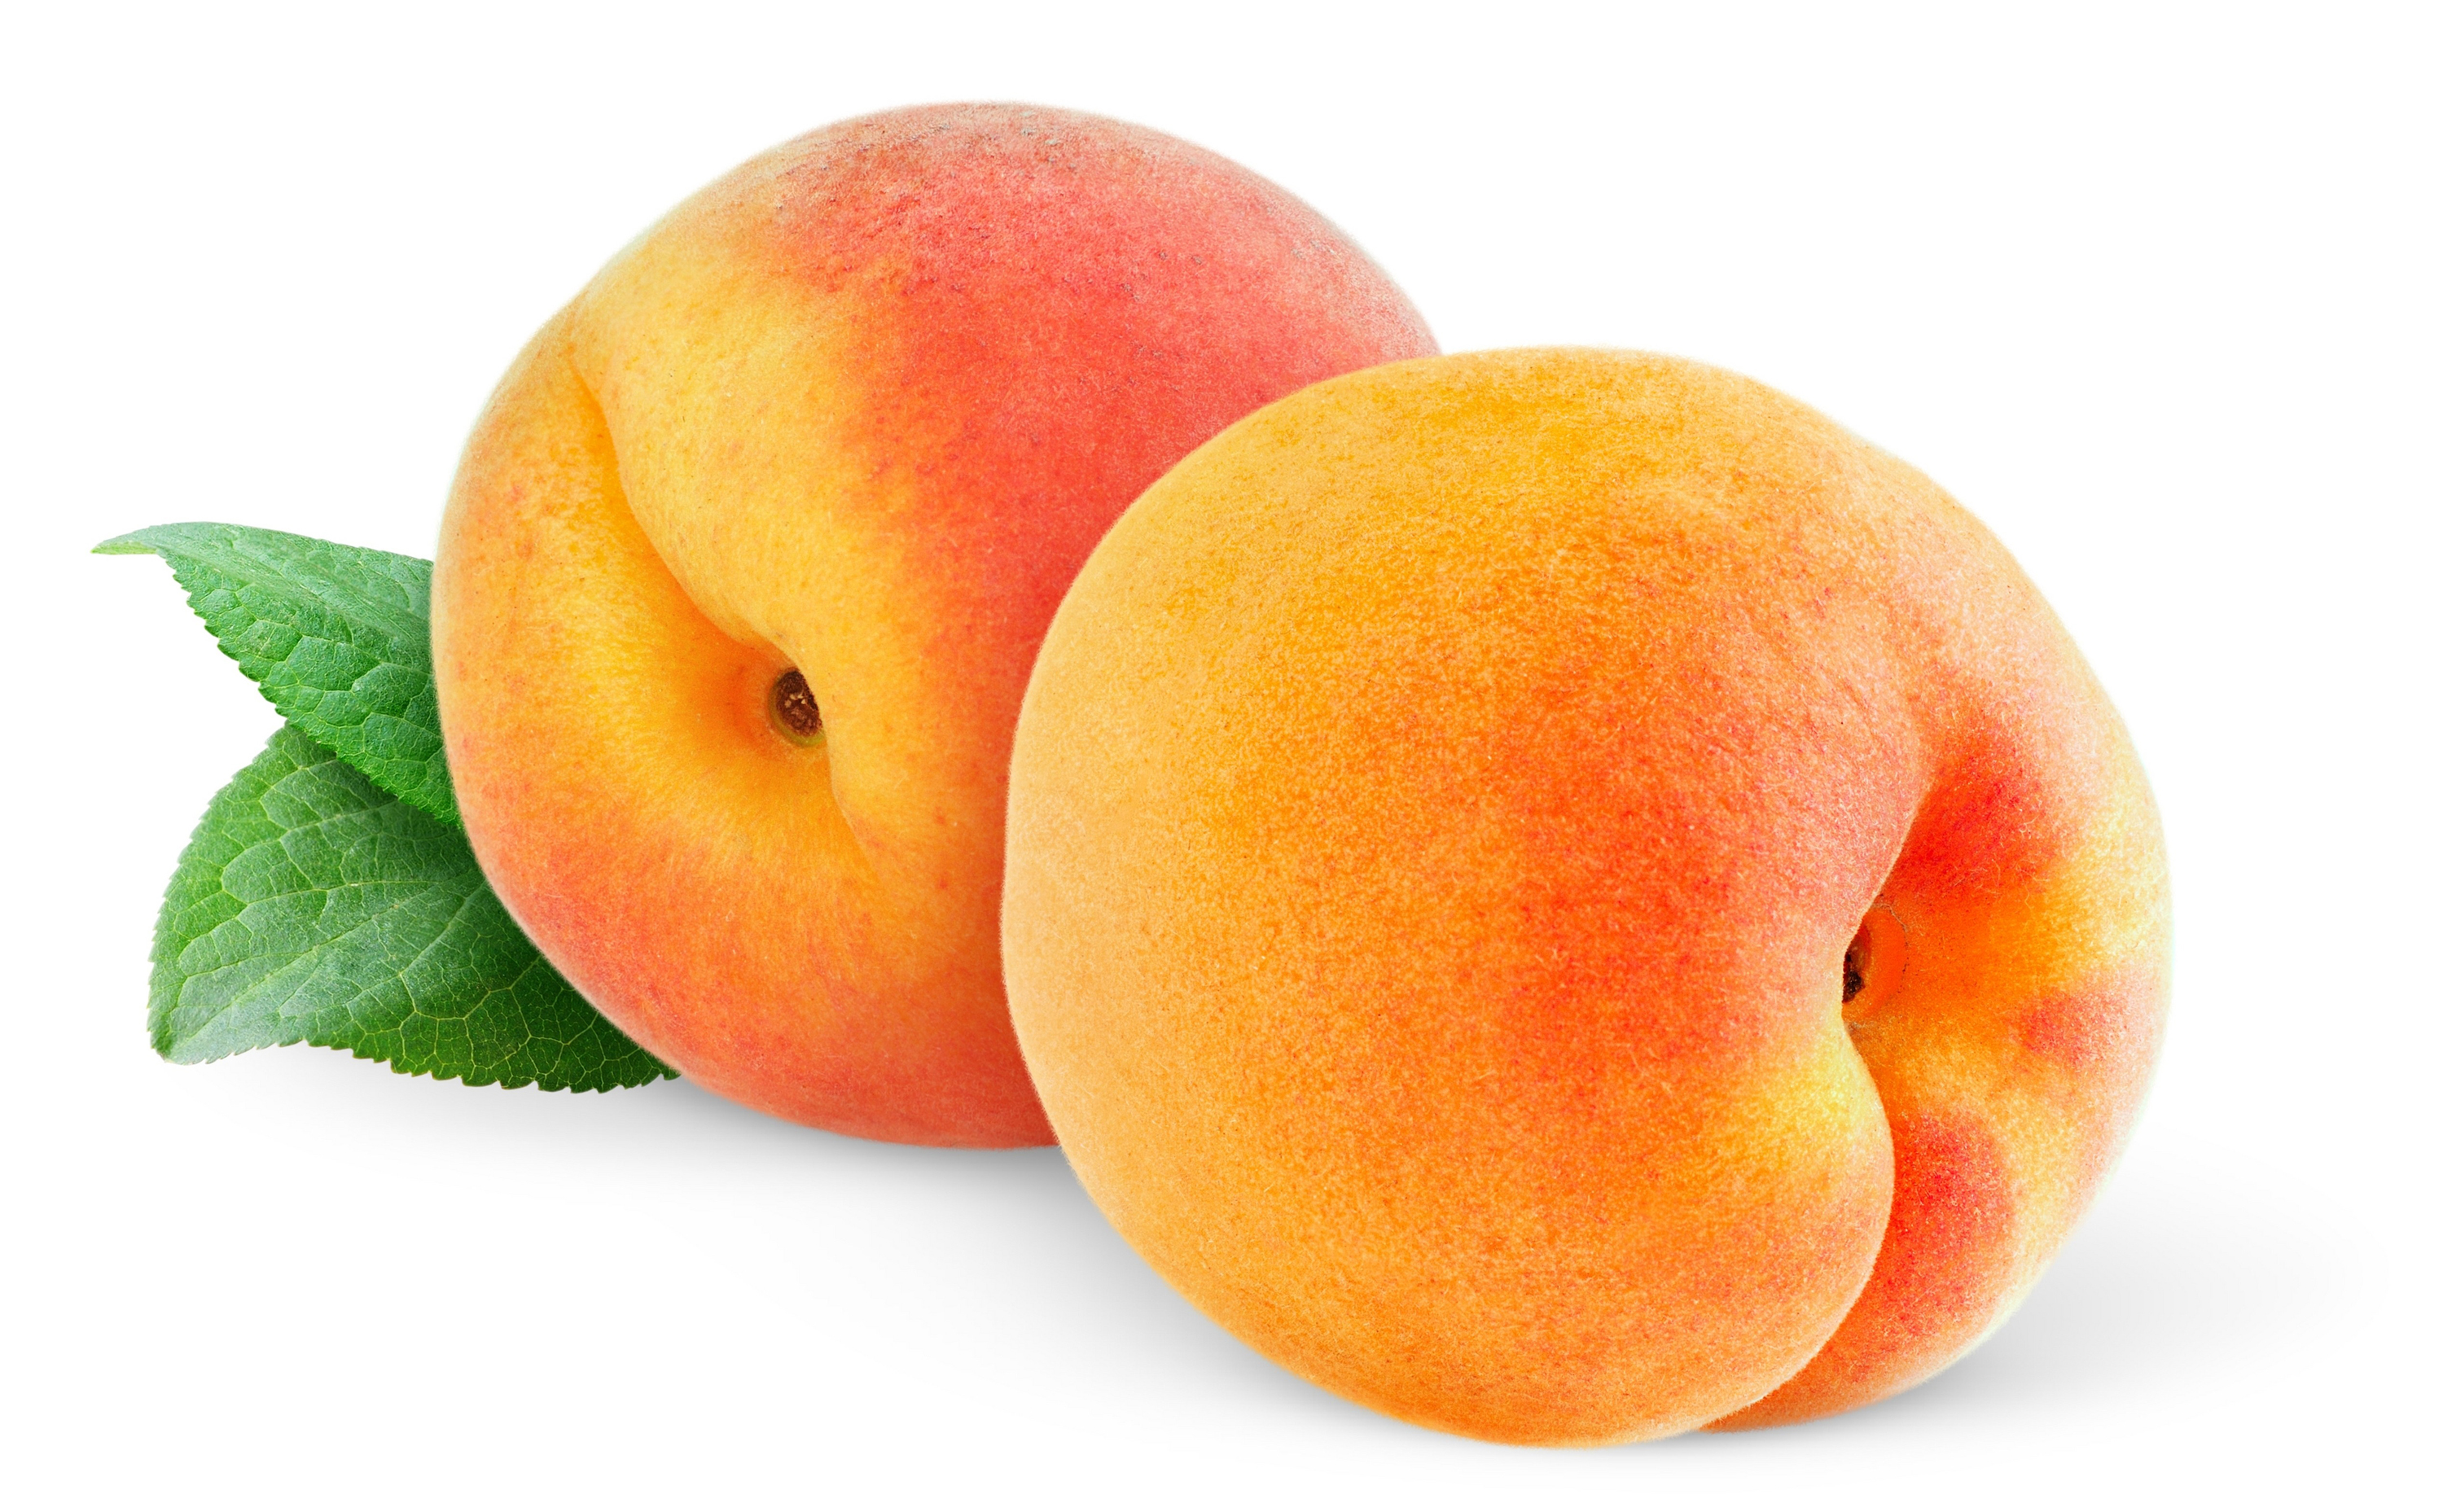
\includegraphics[width=0.8\textwidth]{peachzdfgad.jpg}
  \caption{Delicious peaches although the really new stuff in the paper will be about almonds}
  \label{fig:peach}
\end{figure}



\subsection*{Analysis}
sickle, scythe, bwa-mem, samtools, bcftools...\\
sickle, scythe, bwa-mem, samtools (merge bams), PopBAM, sweepfinder\\
R\\
scripts\\

\section*{Results}


\section*{Discussion}

\pagebreak
%\bibliographystyle{apalike} %can use here and not in header
\bibliography{references.bib}

\pagebreak

\section*{Supplementary Data}
%somehow change table number also maker table width match full width of text
\begin{center}
\begin{longtable}{lllll}
\caption[P. dulcis, P. persica and related species used in analysis.]{P. dulcis, P. persica and related species used in analysis.} \label{my-label} \\
\hline \hline \multicolumn{1}{l}{\textbf{Sample ID}} &
\multicolumn{1}{l}{\textbf{Accession and/or Cultivar}} &
\multicolumn{1}{l}{\textbf{Origin}} &
\multicolumn{1}{l}{\textbf{Source}}  &
\multicolumn{1}{l}{\textbf{Reference}} \\ \hline 
\endfirsthead

\multicolumn{5}{r}{{\bfseries \tablename\ \thetable{} -- continued from previous page}} \\
\hline \multicolumn{1}{l}{\textbf{Sample ID}} &
\multicolumn{1}{l}{\textbf{Accession and/or Cultivar}} &
\multicolumn{1}{l}{\textbf{Origin}} &
\multicolumn{1}{l}{\textbf{Source}} &
\multicolumn{1}{}{\textbf{Reference}} \\ \hline 
\endhead

\hline \multicolumn{5}{r}{{Continued on next page}} \\ \hline
\endfoot

\hline \hline
\endlastfoot

                 \multicolumn{5}{l}\emph{P. dulcis}  \\
                 %PD01 &DPRU 2578.2 & &NCGR &this study\\ %Almond Board resequencing (BGI)
                 PD02 &‘Tardy Nonpareil’ &USA &UCD &this study\\ %Almond Board resequencing (BGI)
                 PD03 &DPRU 1791.3, BE-1609 & &NCGR &this study\\ %Jastro resequencing (performed at UC Berkeley)
                 PD04 &DPRU 2374.12 & &NCGR &this study\\ %Jastro resequencing (performed at UC Berkeley)
                 PD05 &DPRU 1456.4, Badam & &NCGR &this study\\ %Jastro resequencing (performed at UC Berkeley)
                 PD06 &DPRU 2301, Tuono &Italy &NCGR &this study\\ %Jastro resequencing (performed at UC Berkeley)
                 PD07 &DPRU 1462.2 & &NCGR &this study\\ %Jastro resequencing (performed at UC Berkeley)
                 PD08 &DPRU 1207.2 & &NCGR &this study\\ %Jastro resequencing (performed at UC Berkeley)
                 PD09 &DPRU 2331.9 & &NCGR &this study\\ %Jastro resequencing (performed at UC Berkeley)
                 PD10 &DPRU 0210, Languedoc &France &NCGR &this study\\ %Jastro resequencing (performed at UC Berkeley)
                 PD11 &S3067 & &SRR765861 &\citealt{koepke2013comparative}?\\
                 PD12 &D05-187 & &SRR765850 &\citealt{koepke2013comparative}?\\
                 PD13 &Lauranne & &SRR765838 &\citealt{koepke2013comparative}?\\
                 PD14 &Ramillete & &SRR765679 &\citealt{koepke2013comparative}?\\
                 PD{\color{red}15} &Nonpareil & USA&RosBREED &URL \\
                 \\
                 \multicolumn{5}{l}\emph{P. persica}  \\ % format italics
                 %PP01 &Lovell & &SRR502985 &\citealt{verde2013high}\\
                 % doubled haploid
                 PP02 &Yumyeong &Korea? &SRR502994 &\citealt{verde2013high}\\
                 PP03 &Shenzhou Mitao&China &\multirow{2}{1cm}{SRR502993, SRR502992} &\citealt{verde2013high}\\
                 %honey peach
                 \\
                 PP04 &Sahua Hong Pantao &China &\multirow{2}{1cm}{SRR502991, SRR502990} &\citealt{verde2013high}\\
                 %flat peach
                 \\
                 PP05 &Quetta & &\multirow{2}{1cm}{SRR502989, SRR502987} &\citealt{verde2013high}\\
                 \\
                 PP06 &Oro A & &SRR502986 &\citealt{verde2013high}\\
                 PP07 &IF7310828 & &\multirow{2}{1cm}{SRR503001, SRR503000} &\citealt{verde2013high}\\
                 \\
                 PP08 &GF305 & &SRR502983 &\citealt{verde2013high}\\
                 PP09 &Contender $\times$ Ambra & &SRR502997 &\citealt{verde2013high}\\
                 % peach x nectarine both P. persica
                 PP10 &Earligold &USA &\multirow{2}{1cm}{SRR502996, SRR502995} &\citealt{verde2013high}\\
                 \\
                 PP11 &Bolero & &SRR501836 &\citealt{verde2013high}\\
                 PP12 &F8,1-42 &USA &SRR068361 &\citealt{ahmad2011whole} \\
                 PP13 &Georgia Belle &USA &SRR068359 &\citealt{ahmad2011whole} \\
                 PP14 &Dr. Davis &USA &SRR068360 &\citealt{ahmad2011whole} \\
                 PP15 &Lovell &USA &UCD &this study\\
                 %(originally a canning variety selected ~1882, curr rootstock) - FPS, ABC
                 %PP &Lovell & &RosBREED &URL \\
                 %originally a canning variety selected ~1882, currently used as rootstock and/or control for disease screening
                 %downloaded?
                 %duplicate cultivar
                 PP{\color{red}X} &DPRU 0589, Early Crawford&USA &RosBREED &URL \\
                 %introduced before 1832
                 PP{\color{red}X} &DPRU 0941, St. John Yellow &USA &RosBREED &URL \\
                 %introduced 1860s
                 PP{\color{red}X} &DPRU 1190, Admiral Dewey&USA &RosBREED &URL \\
                 %aka PI 673525; introduced 1899
                 PP{\color{red}X} &DPRU 2142, Carmen &USA? &RosBREED &URL \\
                 %PI 673586; cultivar original PI 34673 assigned 1912
                 PP{\color{red}X} &DPRU 2179, Slappey &USA &RosBREED &URL \\
                 %aka ‘Slappy’ in GRIN; introduced 1903
                 PP{\color{red}X} &Babcock&USA &RosBREED &URL \\
                 %not yet downloaded
                 %introduced 1897
                 PP{\color{red}X} &Chinese Cling&China &RosBREED &URL \\
                 %introduced 1850; founder several cultivars
                 PP{\color{red}X} &Diamante&Brazil &RosBREED &URL \\
                 %predominant canning cultivar in Brazil per Okie (year & pub TBD)
                 %not yet downloaded
                 PP{\color{red}X} &Dixon&USA? &RosBREED &URL \\
                 %not yet downloaded
                 %PP &Dr. Davis& &RosBREED &URL \\
                 %not downloaded
                 % duplicate cultivar
                 PP{\color{red}X} &Elberta&USA &RosBREED &URL \\
                 %introduced ~1889; OP sdlg of 'Chinese Cling’
                 PP{\color{red}X} &Florida Prince P138&USA? &RosBREED &URL \\
                 %not yet downloaded
                 %PP{\color{red}X} &Georgia Bell&USA &RosBREED &URL \\
                 %(aka ‘Georgia Belle’ and ‘Belle of Georgia’; introduced ~1875; OP sdlg of Chinese Cling)
                 %not downloaded
                 %duplicate cultivar
                 PP{\color{red}X} &JH Hale&USA &RosBREED &URL \\
                 %male sterile; introduced 1912
                 PP{\color{red}X} &Mayflower&USA &RosBREED &URL \\
                 %introduced 1909
                 %not yet downloaded
                 PP{\color{red}X} &Nemaguard &USA &RosBREED &URL \\
                 %rootstock; rumored to have P. davidiana in pedigree
                 PP{\color{red}X} &O’Henry &USA &RosBREED &URL \\
               %CODE FOR APOSTROPHE
                 %plant patent 2.964 1/27/1970; OP sdlg Merrill Bonanza; discovered 1960
                 %not yet downloaded
                 PP{\color{red}X} &Okinawa &? &RosBREED &URL \\
                 PP{\color{red}X} &Oldmixon Free &USA &RosBREED &URL \\
                 % introduced 1832
                 %not yet downloaded
                 PP{\color{red}X} &Rio Oso Gem &? &RosBREED &URL \\
                 %not yet downloaded
                 %some variety history at http://gapeaches.org/about-us/father-of-the-ga-peach-industry/
                 \multicolumn{5}{l}{} \\
                 \multicolumn{5}{l}{Other \emph{Prunus} species}  \\
                 %Almond Board resequencing (performed at BGI)
                 PF01 &\emph{P. fenzliana} &? &UCD &this study\\
                 %UCD,ABC
                 PG01 &\emph{P. ferganensis} &China? &\multirow{2}{1cm}{SRR502999, SRR502998} &\citealt{verde2013high}\\
                 \\
                 PC01 &\emph{P. cerasifera} DPRU 0579, Myrobalan &? &NCGR &this study\\ \hline
                 %outgroup
                 %NCBI SRA
               %note that the SRR IDs are from NCBI SRA
               %GDR/RosBREED (ftp://ftp.bioinfo.wsu.edu/species/Prunus_persica/RosBREED_Illumina/)

\end{longtable}
\end{center}

\end{document}